\pdfoutput=1 % for arXiv to use pdflatex
\documentclass[12pt]{article}

%% The graphicx package provides the includegraphics command.
\usepackage{graphicx}
%% The amssymb package provides various useful mathematical symbols
\usepackage{amsmath}
\usepackage{amssymb}
%% The lineno packages adds line numbers. Start line numbering with
%% \begin{linenumbers}, end it with \end{linenumbers}. Or switch it on
%% for the whole article with \linenumbers after \end{frontmatter}.
\usepackage{lineno}
\usepackage{url}
\usepackage{xspace,multicol}
\usepackage{siunitx}
\usepackage{subcaption}
\usepackage{color, colortbl}
\usepackage{units}
\usepackage{ragged2e}
\usepackage{array}
\usepackage{tabularx}
\usepackage{authblk}
\usepackage{heppennames}
\usepackage{feynmp}
\usepackage{libertine}
% \usepackage[libertine]{newtxmath}
\usepackage{textgreek}
\DeclareGraphicsRule{*}{mps}{*}{}

\newcommand{\guineapig}{GuineaPig\xspace}
\newcommand{\sid}{SiD\xspace}
\newcommand{\slic}{\textsc{SLIC}\xspace}
\newcommand{\geant}{\textsc{Geant4}\xspace}
\newcommand{\murm}{%
  \ifmmode
    \mathchoice
        {\hbox{\normalsize\textmu}}
        {\hbox{\normalsize\textmu}}
        {\hbox{\scriptsize\textmu}}
        {\hbox{\tiny\textmu}}%
  \else
    \textmu
  \fi
}
\newcommand{\micron}{\ensuremath{\murm\mathrm{m}\xspace}}

\begin{document}

%% Title, authors and addresses

\title{A Study of the Impact of Muons from the Beam Delivery System on the SiD Performance}

\author{Anne Sch\"utz\footnote{Karlsruhe Institute of Technology (KIT), Department of Physics, Institute of Experimental Nuclear Physics (IEKP), Wolfgang-Gaede-Str. 1, 76131 Karlsruhe, Germany}, Marcel Stanitzki\footnote{Deutsches Elektronen-Synchrotron (DESY), Notkestr. 85, 22607 Hamburg, Germany}}

\maketitle

%%
%% Start line numbering here if you want
%%
\linenumbers

\begin{abstract}
%% Text of abstract
To suppress the muon background arising from the Beam Delivery System (BDS) of the International Linear Collider (ILC), and to hinder it from reaching the interaction region, two different shielding scenarios are under discussion: five cylindrical muon spoilers with or without an additional magnetized shielding wall.
Due to cost and safety issues, the case preferred by the MDI group is to omit the shielding wall, which on the other hand brings other disadvantages.
To support the decision making, the impact of the muons from the two different shielding scenarios was studied in a full Geant4 detector simulation of the SiD detector, one of two proposed detectors for the ILC. 
Input to this study is the muon background created by the beam traveling through the BDS, which was simulated with the simulation tool MUCARLO.
\end{abstract}


%% main text
\section{Introduction}
\label{sec:introduction}

The muon background from the BDS arises from the the beam halo hitting the material along the beam line, e.g. the beam collimator systems.
Therefore, the muons are created along the BDS and travel towards the interaction region.
To prevent the muons from reaching the detectors, it is studied which shielding system would be effective and reasonable to be integrated in the BDS.
Several different shielding scenarios have already been under discussion and have been dropped, so that the two cases currently discussed and presented in this proceeding are both yielding acceptable muon rates at the interaction region.
In the first scenario five cylindrical magnetized spoilers are installed at different positions along the beam line.
The second scenario adds a magnetized iron wall close to the interaction region.
Both, the spoilers and the wall are shown in schematic drawings in Figure~\ref{fig:Spoilers_Wall}.
Their location in the BDS can be seen in Figure~\ref{fig:Spoilers_Wall_Locations}.
\begin{figure}
    \centering
    \begin{subfigure}[b]{0.53\textwidth}
        \includegraphics[width=\textwidth]{figures/Spoiler.png}
        \caption{The magnetized iron spoilers}
	\label{fig:spoilers}
    \end{subfigure}
    \begin{subfigure}[b]{0.42\textwidth}
        \includegraphics[width=\textwidth]{figures/Muon_wall.pdf}
        \caption{The magnetized iron wall}
        \label{fig:wall}
    \end{subfigure}
    \caption[Schematic drawings of the shielding systems]{
    Schematic drawings of the magnetized cylindrical spoilers and the magnetized wall.
    The spoilers have a radius of \unit{70}{cm} and a length of \unit{5}{m}, while the wall is about \unit{5}{m} long and wide and fills out the entire tunnel height.
    }
    \label{fig:Spoilers_Wall}
\end{figure}

\begin{figure}
    \centering
    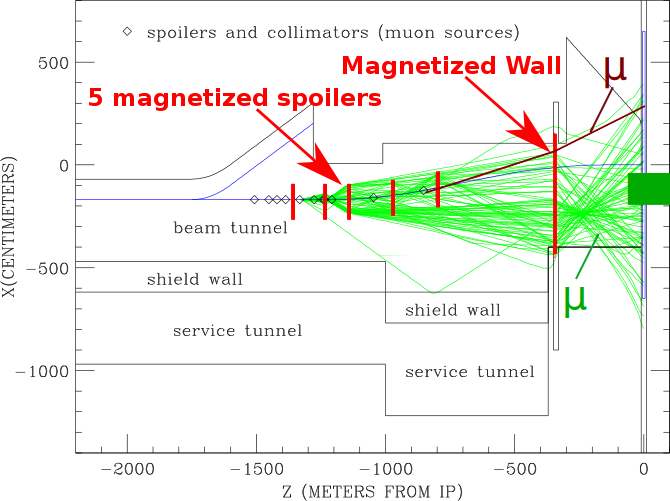
\includegraphics[width=0.7\textwidth]{figures/BDS_Tunnel_Spoilers+Wall.png}
    \caption[BDS tunnel with the spoiler and wall positions]{
    The five spoilers are located at the following positions along the BDS tunnel: \unit{802.5}{m}, \unit{975.5}{m}, \unit{1145.5}{m}, \unit{1234.5}{m}, and \unit{1358.5}{m}.
    For the second shielding scenario, the wall would be additionally installed at \unit{400}{m} away from the interaction point.
    }
    \label{fig:Spoilers_Wall_Locations}
\end{figure}

Due to the size of the wall which causes cost and safety issues, the MDI group prefers the first scenario without the wall.
What has to be kept in mind on the other hand is that the wall reduces not only the muon rate but also shields the neutron and photon background created by the machine.
Not having this shielding wall would therefore mean no access to the interaction region when the beam is on, i.e. the access to the detector in the garage position will not be allowed.


SiD requirements for low background


\section{The Simulation of the Muon Background with MUCARLO}
\label{MUCARLO}

The simulation code MUCARLO\cite{MuonBkg_05TeV, MuonBkg_1TeV} is based on Fortran, and was originally written by Gary Feldman.
Over the years it has been expanded, and is used in several studies, from the study of muon shielding designs for radiation protection, to fixed target experiments at SLAC and muon background simulation studies for the Next Linear Collider (NLC) and the ILC\cite{MuonBkg_05TeV, MuonBkg_1TeV}.\\
For the presented study, the Technical Design Report (TDR) baseline machine parameters for the ILC-500GeV are used for simulating the beam interacting with the BDS geometry and the muon collimation system.
The muons are produced in interactions of the beam halo with material in the beam lines, in which the predominant interaction is the Bethe-Heilter process:
\textgamma + Z $\rightarrow$ Z' + \murm\textsuperscript{+}\murm\textsuperscript{-}\\
The muon production by direct annihilation of the positrons with atomic electrons is also taken into account.\cite[sec. 2]{Mucarlo}
For tracking the beam halo, the tool TURTLE\cite{Turtle} is used.\\
The results from the MUCARLO simulations can be seen in Table~\ref{tab:MuonRates}, listing the number of muons reaching the interaction region for the two shielding scenarios and for the case of not having any muon shielding system.
The calculated muon rate is based on a halo population of 10\textsuperscript{-3}, which is more than ten times larger than expected from ring scattering calculations.
This estimation corresponds to the worst halo measured at the Stanford Linear Collider (SLC), and is therefore used as a worst-case scenario.

\begin{table}
\caption{MUCARLO results: The number of muons hitting a detector with radius of \unit{6.5}{m} in the different shielding scenarios.}
\label{tab:MuonRates}
\centering
\begin{tabularx}{\textwidth}{ll}
\hline\hline
\textbf{Scenario} & \textbf{Number of muons in a detector with 6.5m radius}\\
\hline
\cline{1-2}
\hline
 No Spoilers & 130 muons/bunch crossing\\
 5 Spoilers& 4.3 muons/bunch crossing\\
 5 Spoilers + Wall & 0.68 muons/bunch crossing\\
\hline\hline
\end{tabularx}
\end{table}
\section{The simulation of muons in the SiD detector}
\label{Detector}

In the first step of simulating the muons in the SiD detector, event displays were made with WIRED4.

\begin{figure}
    \centering
    \begin{subfigure}[b]{0.49\textwidth}
    \centering
        \includegraphics[height=0.3\textheight]{figures/muons_positron_5spoilers_wall_515_xyview_croped.png}
        \caption{xy-view}
	\label{fig:xy_5Spoilers}
    \end{subfigure}
    \begin{subfigure}[b]{0.49\textwidth}
    \centering
        \includegraphics[height=0.3\textheight]{figures/muons_positron_5spoilers_wall_515_zyview_croped.png}
        \caption{xy-view}
        \label{fig:zy_5Spoilers}
    \end{subfigure}
    \caption[Event displays of muons in SiD from the '5 Spoilers' scenario]{
    Event displays in the xy- and zy-view of the muons from the '5 Spoilers' scenario in the SiD detector.
    }
    \label{fig:WIRED4_5Spoilers}
\end{figure}

\begin{figure}
    \centering
    \begin{subfigure}[b]{0.49\textwidth}
    \centering
        \includegraphics[height=0.3\textheight]{figures/muons_positron_5spoilers_2961_xyview_croped.png}
        \caption{xy-view}
	\label{fig:xy_5SpoilersWall}
    \end{subfigure}
    \begin{subfigure}[b]{0.49\textwidth}
    \centering
        \includegraphics[height=0.3\textheight]{figures/muons_positron_5spoilers_2961_zyview_croped.png}
        \caption{xy-view}
        \label{fig:zy_5SpoilersWall}
    \end{subfigure}
    \caption[Event displays of muons in SiD from the '5 Spoilers + Wall' scenario]{
    Event displays in the xy- and zy-view of the muons from the '5 Spoilers + Wall' scenario in the SiD detector.
    }
    \label{fig:WIRED4_5SpoilersWall}
\end{figure}
\section{Summary and conclusion}
By looking at the luminosity spectra generated for this study, the expected rise in luminosity for the proposed ILC250 parameter sets is confirmed.
The total luminosity resulting from the new official beam parameter set (A) is increased by about \SI{97}{\percent} with respect to the original beam parameters, leading to a new value of \SI{1.62e34}{\per\centi\meter\squared\per\second}.
The background studies indicate that the new beam parameters increase the \Pep\Pem pair background density and the SiD vertex detector occupancy by only a factor of about 2-3 in comparison to the original TDR beam parameters.
As for a precision detector the aim is to keep the overall ratio of so-called ``dead'' cells with a full buffer below a per mill level, any rise in the occupancy level can be critical.
Although the density of the pair background close to the interaction point rises, the normalized vertex detector occupancy for the new set is well below 10$^{-4}$.
The highest occupancy is reached in the innermost layer with a fraction of dead cells of about \num{5e-5}, assuming a buffer depth of four.\\
The SiD Optimization group is confident that this rise in the occupancy can be accommodated in the design of the SiD vertex detector without a loss in precision for the physics studies.
Therefore, the SiD group welcomes the decision to change the beam parameters in order to gain higher luminosities and to strengthen the physics program.


\section*{Acknowledgments}
Grateful acknowledgments to Lewis Keller and Glen White from SLAC for the simulation of the muons from the BDS and their big support.

\include{Appendix}

%% References with bibTeX database:

\bibliographystyle{abbrv}
%\bibliographystyle{model1-num-names} %Doesn't work well if you also cite webpages (Confluence page)
\bibliography{bibliography.bib}

\end{document}
